\chapter{Results and Discussion}
\label{chap:results}
\begingroup
\justifying
\setlength{\parindent}{2em}
\setlength{\parskip}{0.55\baselineskip}

\section{Reading the results}

Three kinds of evidence appear in this chapter and they answer different questions.

Scene and simulation measurements say whether the generated stores are usable at all---whether a plan can be built, instantiated and stepped quickly enough to run an experiment on. Demonstration and interface results say whether one adaptation pipeline can be laid across four architectures that share almost nothing internally. Policy success rates and failure labels describe the four trained pipelines under the protocol that was actually executed. Only the third body of evidence concerns policy behaviour, and even there the model, adaptation recipe and execution setup remain entangled.

Keeping the three apart matters more than it sounds. A benchmark project can run as designed and still return nothing but low numbers. Those numbers describe the evaluated pipelines, not architecture quality; nor do they prove that every part of the implementation is faultless. Much of this chapter locates that boundary.

\ref{tab:main-results} carries the policy comparison. Every task--item--fixture triplet contains a hundred trials. Under Pose and Layout, Basket and Board pool 300 trials per task-level cell, while Floor, Open and Close pool 200. Under Pairing, each applicable pick-and-place task pools two held-out product triplets, hence 200 trials. A dash marks a condition the door tasks do not have. It is not a zero. The two composite columns are zero for every model and every scenario. One historical $\pi_0$ Pairing aggregate cannot be reconstructed from the archived product-level outcomes and is marked NR rather than treated as a count.

\begin{table}[H]
\centering
\scriptsize
\setlength{\tabcolsep}{2.2pt}
\resizebox{\textwidth}{!}{%
\begin{tabular}{llrrrrrrrr}
\toprule
Model & Scenario & Basket & Floor & Board & Open & Close & Pick 3 & Fridge seq. \\
\midrule
\multirow{3}{*}{Octo}
 & Pose & 1 & 1 & 2 & 3 & 4 & 0 & 0 \\
 & Layout & 2 & 1 & 1 & 2 & 7 & 0 & 0 \\
 & Pairing & 0 & 0 & 0 & -- & -- & 0 & 0 \\
\midrule
\multirow{3}{*}{SmolVLA}
 & Pose & 0 & 0 & 0 & 1 & 2 & 0 & 0 \\
 & Layout & 0 & 0 & 0 & 1 & 2 & 0 & 0 \\
 & Pairing & 0 & 0 & 0 & -- & -- & 0 & 0 \\
\midrule
\multirow{3}{*}{$\pi_0$}
 & Pose & 1 & 1 & 1 & 2 & 2 & 0 & 0 \\
 & Layout & 1 & 1 & 1 & 2 & 2 & 0 & 0 \\
 & Pairing & 0 & NR$^{\dagger}$ & 0 & -- & -- & 0 & 0 \\
\midrule
\multirow{3}{*}{$\pi_{0.5}$}
 & Pose & 1 & 1 & 1 & 2 & 2 & 0 & 0 \\
 & Layout & 1 & 1 & 1 & 1 & 2 & 0 & 0 \\
 & Pairing & 1 & 1 & 3 & -- & -- & 0 & 0 \\
\bottomrule
\end{tabular}}
\caption{Task-level success rates (\%). Every task--item--fixture triplet contains 100 trials. For Pose and Layout, Basket and Board pool three triplets (300 trials), while Floor, Open and Close pool two (200 trials). Pairing pools two held-out product triplets (200 trials) for each applicable pick-and-place task and is undefined for the doors. Successes are summed across equal-sized triplets before division; displayed percentages are rounded to the nearest whole percentage point using round-half-up, while unrounded numerators and denominators govern all calculations. The door-task Layout condition reuses the training plans and changes only texture and starting pose. ``Basket'', ``Floor'' and ``Board'' abbreviate the three pick-and-place tasks. $^{\dagger}$The archived task-level record reports a rounded 1\% for this cell, but the product-level outcomes and unrounded numerator were not retained; it is therefore reported as not recoverable and excluded from count-based calculations.}
\label{tab:main-results}
\end{table}

One thing the table deliberately does not do is collapse. Averaging a door-closing score against a shelf-picking score produces a number, and the number means nothing: the two tasks succeed and fail for unrelated reasons. Reading down a column shows the recorded task-level rates; reading across a row shows the point estimates under each condition. A single overall score would preserve neither distinction.

\section{RQ1: scene generation and computational usability}

RQ1 asked for variation without loss of structure, and on the operational half of that question the pipeline delivers. Different seeds give different store plans rather than reshuffles of one room. Each plan serialises to JSON under a configuration hash, instantiates in ManiSkill3 and keeps its aisles open. Fixtures come out in coherent runs---rows of three to five units placed end to end, with free space between them---rather than scattered across the floor, as \ref{fig:store-generation} shows.

That structure deserves a careful sentence, because the mechanism producing it is coarser than the equations in the system chapter on their own suggest. Every shelf is axis-aligned. What the field decides is where one may sit, not which way it points, and with a decay coefficient of 12 that decision falls to whichever wall or fixture contour happens to lie within about thirty centimetres. The rows are real. They come from a gate applied along a sweep, not from continuous alignment to a smoothly blended orientation.

Product placement contributes controlled visual density but not depletion. The depletion mechanism has no counterpart in the implementation and generated no scene in this study: every shelf in training and evaluation is fully packed. The distinction matters because a designed capability and an exercised one are not the same evidence.

\ref{fig:mesh-performance} records the computational test used for RQ1. Fifty simulation steps were timed on one RTX 4090 while the number of stocked shelving units increased. The original-mesh series rises from 0.21~seconds at one unit to 1.24 at four, where the recorded series ends. The simplified series includes scenes from one to 118 units and remains between 0.23 and 0.42~seconds at the four sampled sizes.

The result is useful but not a matched speed-up estimate. No repeated measurements or original-mesh points above four units were retained, and the 118-unit comparison changes scene size together with mesh detail. At one unit, simplified geometry is actually slower. The defensible conclusion is therefore practical: the recorded setup stepped a densely stocked 118-unit scene with simplified assets, whereas the original-mesh test was not continued beyond four.

\begin{figure}[H]
    \centering
    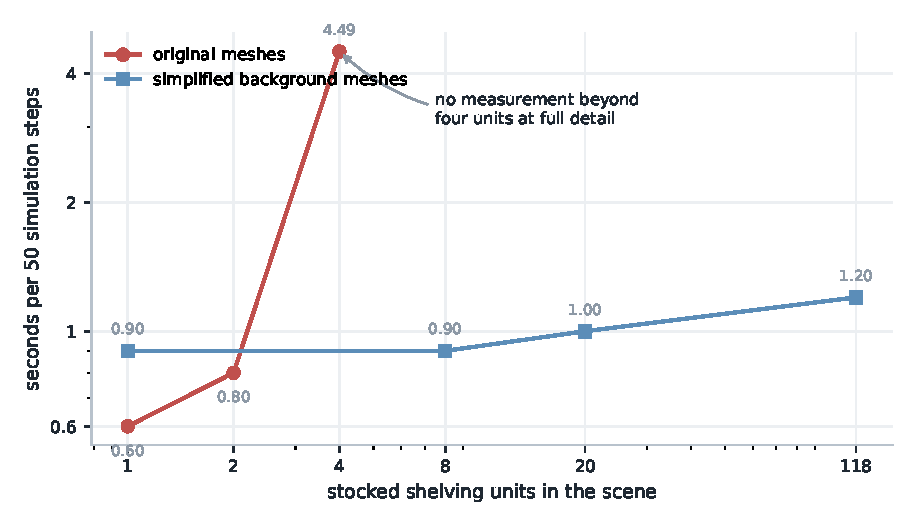
\includegraphics[width=0.68\textwidth]{assets/figures/retail-vla-benchmark/mesh_timing.pdf}
    \caption{Time for 50 simulation steps against the number of stocked shelving units, on log--log axes. The original-mesh series ends at four units, beyond which the scene was impractical to step; the simplified series stays near 0.4~s from one unit to 118. Below roughly two units the original meshes are the faster option, so the two series cross rather than separate.}
    \label{fig:mesh-performance}
\end{figure}

A separate throughput sweep compared state and RGB observations across parallel environments. Its raw result files were not retained, so the apparent saturation of rendered throughput is treated here as a study note, not as a quantitative result. Capacity planning, exact frame-rate claims and memory ratios require the sweep to be rerun from the recorded procedure.

RQ1 is answered for generation and computational cost. Its remaining criteria require narrower conclusions: the scenes were intended to be collision-free, navigable and visually plausible.

Collision-free placement holds by construction, since a candidate that fails the footprint or passage test is never accepted. Visual plausibility was inspected by the author but not measured through a realism study, comparison with surveyed store-plan distributions or physical validation. Navigability was established only as geometric passage provision: the plans leave two metres of clearance and support base motion, but no reported episode required store-scale navigation because each begins 1.4~metres from the relevant fixture. Section~\ref{sec:verification} returns to that limitation.

A generator can therefore be judged sound on the criteria it was built against while leaving the most interesting of those criteria untested. That is the position here.

\section{RQ2: demonstration generation and adaptation}

The collection covers twelve task--item--fixture triplets: 248 successful episodes apiece, 2,976 trajectories and 1,401,169 transitions. It took about ten hours of wall-clock time on a single RTX 4090. Anchor decomposition with screw motion and an RRT-Connect fallback reached that without anyone touching a teleoperation rig, and one observation--action schema then fed four model families whose internals have almost nothing in common. As a supervision source, the pipeline does what it was built to do.

Two things about the corpus are thinner than the totals imply. The layout pool behind it is smaller than the documentation states, because two configuration files meant to generate different stores for board transfer were given the same seed, as were the two for floor recovery; those tasks draw on five distinct plans rather than ten. And the fallback structure is less redundant than the methodology chapter describes---the second screw attempt repeats the first call with identical arguments, which for a deterministic solver cannot change anything. Neither issue costs a result. Both narrow what ``scalable and diverse'' is entitled to mean here.

The more revealing comparison sits in the appendix rather than the main table, and it is the one between Seeds and Pose. Nothing about the scene changes between those two columns. The store is the same store; the shelf holds the same products in the same places; and the instruction is word for word what it was during collection. All that moves is where the robot happens to be standing when the episode starts. The bounds differ by task and neither is large: roughly twenty centimetres of retreat and a quarter of a metre sideways for basket picking, a little under half a metre on both axes for board transfer, with about twenty-two degrees of yaw in either case.

Octo goes from 5\%, 3\% and 3\% on its three board-transfer products to 3\%, 1\% and 1\%. $\pi_{0.5}$ goes from 2\%, 2\% and 2\% on pick-to-basket to 1\%, 1\% and 1\%.

The direction is the one the comparison was built to expose, and the magnitude is too small to build on. Two episodes in a hundred separate Octo's best board-transfer product between Seeds and Pose under a perturbation bounded a little below half a metre on each horizontal axis. In a future convergence-checked run with measurable rates, this comparison would be the sharpest instrument in the chapter, because it needs no argument about what counts as a distribution shift---nothing about the scene changes at all. In the present fixed-step run it is a column of single-digit counts moving by one or two, and it is reported here as a measurement that the protocol supports rather than as a finding the data can carry.

SmolVLA is the one row where the shape survives its own smallness. It records zero on every reported pick-and-place product, in every condition, including the training seeds, while still opening and closing refrigerated and showcase fixtures at rates between 1\% and 4\%. A model that never once places a product in the basket it was shown 248 times, but does occasionally move a door, is not failing uniformly. Whether that pattern would persist under a convergence-checked training configuration is exactly what this study cannot establish.

The present fixed-step configuration does not reveal why this happened. Capacity, pretraining mixture, action normalisation, low-rank adaptation and checkpoint choice remain confounded. At rates this low, success-rate contrasts say little about the underlying model families, even though the failed rollouts still expose where the evaluated pipelines stop.

RQ2 divides cleanly, and the two halves deserve separate answers. On demonstration generation it is answered yes: the pipeline produced 2,976 successful trajectories and 1,401,169 transitions from task specifications without a teleoperation rig, and a single observation--action schema fed four architectures with almost nothing in common. On adaptation it is answered only in the weakest sense available. In the triplet-level Seeds/Pose/Layout table---four models by three modes by twelve task--item--fixture combinations---111 of 144 cells contain at least one success; Pairing and composite-task cells are not included in that count. The four fixed-step configurations nevertheless did not produce dependable behaviour. Because training sufficiency was not established, this study cannot determine whether the corpus suffices for adaptation or isolate the effects of data, compute, optimisation and task difficulty.

Part of the reason is visible in what the collector keeps. It keeps successes, and only successes. The policy learns what a nominal planned trajectory looks like; it receives less evidence about how to correct a base error or reattempt a missed grasp. The prevalence of pre-grasp and grasp failures is consistent with this limitation, although the present experiments do not prove a causal link.

They also do not rule out a competing account, which Section~\ref{sec:failure-modes} returns to. The evaluation client requests a fifty-step action chunk and executes all of it before constructing the next observation, so a policy sees the scene between ten and twenty times across a whole episode and spends the intervening steps committed to a plan it cannot revise. Missing recovery data and missing opportunity to recover produce the same failure label.

\section{RQ3: atomic-task performance}
\label{sec:atomic}

No model achieves dependable task success under the training configuration evaluated here. That sentence is the result, and everything else in this section is an argument about what may and may not be read into it.

The triplet-level Seeds/Pose/Layout table in Appendix~\ref{app:training-results} contains four models, three modes and twelve task--item--fixture combinations: 144 cells in total. Pairing and composite-task cells are not included in that count. The table spans zero to nine successes in a hundred trials, with a mean of 1.5, and 111 cells contain at least one success. The single best cell is Octo closing a showcase door at 9\%. Under Pose, no model exceeds 4\% on any task. The policies are therefore not inert, but the retained outcomes do not support the comparisons this chapter was designed to make.

The limitation on interpretation is stated in Section~\ref{sec:training}. Every model was adapted on one RTX 4090 at batch size 8, for between 30,000 and 100,000 steps, and three of the four through low-rank updates rather than full fine-tuning. No learning-rate or schedule search was carried out. Each run stopped when its preset counter expired, and none was assessed with a validation-based convergence criterion. What \ref{tab:main-results} measures is what these four study pipelines achieved after a few hours of single-card adaptation. That is a legitimate question. It is not the same as asking how well the underlying architectures can learn retail manipulation.

The consequence for interpretation is severe and worth stating in arithmetic rather than in hedging. A hundred trials were run for each item--task--scenario triplet, so a 1\% triplet entry is one successful episode and a 4\% entry is four. The task-level cells pool 200 or 300 trials, depending on scenario and task, and all calculations use the underlying counts rather than the displayed integer percentages. Marginal Wilson intervals could describe uncertainty for an individual pooled rate under an independent-Bernoulli assumption. They are not tests of a model, task or condition contrast, and overlap between two such intervals is not used here as a significance rule. The retained aggregates also omit the episode pairing and grouping needed for design-aware contrasts across shared configurations, items and layouts. Architecture and task rankings are therefore unsupported: adaptation recipes are unmatched, success predicates differ, and item and layout variation has not been modelled.

Three claims a reader may expect from the surrounding literature are worth checking against this table and finding absent. That articulated doors are easier than shelf picking: not supported here---door and pick-and-place columns are separated by two or three episodes. That floor recovery is anomalously hard: not supported---it sits at the floor along with everything else, and under the Seeds condition Octo's highest task mean is in fact floor recovery at 7.5\%. That one policy family transfers better than another: not supported, and Section~\ref{sec:results-shift} explains why the shift comparison cannot be run at all from this baseline. None of the three is refuted by these results; each is simply beyond what they can reach.

One asymmetry is large enough to note without resting anything on it. Octo, the smallest model at 93M parameters and the only one fully fine-tuned rather than adapted through low-rank updates, produces the highest numbers in the table. Whether that reflects the architecture, the smaller parameter count fitting the budget better, or full fine-tuning being the more effective use of a fixed number of steps, this experiment cannot say, since adaptation method and model scale move together across the four rows. It is recorded here as an observation with an experiment attached rather than as a finding.

\section{Distribution shift}
\label{sec:results-shift}

The observed Pose--Layout differences can be calculated from the pooled counts, but they do not answer the transfer question on their own.

The rounded percentages in \ref{tab:main-results} hide several fractional movements, so the comparison has to return to those counts. Ten of the twenty model--task pairs are exactly unchanged from Pose to Layout. Nine move by between one third and two thirds of a percentage point in magnitude. The remaining pair, Octo on door closing, rises from 8/200 to 13/200: five additional episodes, or 2.5 percentage points. Pose success is only 0--4\%, which sharply limits the observable downward range. The retained aggregates also do not permit a design-aware interval for each condition contrast. For the doors, the nominal Layout condition is narrower still because it changes texture and starting pose but not scene geometry.

The distinction between no observed loss and evidence of no loss matters here. A study with a reliable in-domain baseline could estimate a change under a new store plan and attach uncertainty to that contrast. Here the strong floor effect and incomplete statistical record prevent the data from distinguishing a small degradation from no change or improvement. The pick-and-place shift conditions are built and runnable; the door condition does not implement the intended geometric shift. The resulting point differences are reported, but they are not treated as a transfer estimate.

Pairing is the one condition where something is still visible, and only because it is bounded below. Octo and SmolVLA record zero on all three applicable tasks. A historical task-level record gives a rounded 1\% for $\pi_0$ on floor recovery, but the archived product-level outcomes and unrounded numerator were not retained; the cell is therefore marked NR and excluded from count-based comparisons. $\pi_{0.5}$ records 1\% on pick-to-basket, 1\% on floor recovery and 3\% on board transfer; only the board-transfer figure exceeds its corresponding Seeds mean. What can be said is that the two smaller policies reach exact zero when the target product is one they were never asked to handle on that task. That pattern is consistent with a grounding failure, but it is not evidence for one.

Whether current generalist policies transfer across retail-specific geometric and semantic shift remains unanswered in either direction. The study established the conditions, generated the scenes and ran the protocol, but the floor-limited baseline and retained aggregate record do not distinguish a small degradation from no change or improvement. Section~\ref{sec:ablations} sets out the convergence-checked comparison needed before that question can be answered.

One property of the setup remains worth stating because it bounds the question independently of the training budget. It is tempting to explain any Layout effect partly through changed navigation geometry, since the layout moves and the aisles move with it. Episode initialisation sharply limits that reading. The robot is placed 1.4~metres in front of the correct fixture and turned to face it at the start of every episode, in every condition. Basket and Floor then perturb translation by roughly a quarter of a metre per axis; Board uses bounds a little under half a metre; all three use a yaw range of about twenty-two degrees. Nothing in the reported protocol asks a policy to cross a store or to choose between distant fixtures. Even with a budget sufficient to produce measurable rates, the pick-and-place Layout contrast tests visual context and the final approach, not store-scale navigation. The door contrast is narrower again because its geometry does not change.

\section{Composite tasks}

Every composite-task entry is zero. This is the clearest result in the table and the easiest to overstate. The evaluation does not show that a model cannot understand a multi-step natural-language request, because an oracle supplies atomic instructions. It shows that none of the tested adapted policies completed the full execution chain under the protocol.

Compounding atomic error provides a strong baseline explanation. If three stages each succeeded with probability 0.5 and were independent, complete success would be 12.5\%. With a 0.2 atomic rate, it would be 0.8\%. The actual stages are dependent: a poor placement may alter camera views or block the next approach, and the robot state after one completion differs from a clean reset. Zero observed success is therefore compatible with the atomic rates without requiring a separate language-planning failure.

The finding still matters operationally. Retail value comes from finished orders, not isolated benchmark primitives. A policy that occasionally picks one item but cannot sustain a short sequence is not ready for unattended fulfilment.

A column of zeros is also an incomplete account of sequential behaviour. Each composite environment exposes a per-subtask completion flag and a normalised progress count alongside binary success. Those episode-level outputs were not retained in the archived results bundle, so partial progress cannot be reconstructed for this dissertation without rerunning evaluation. The reported result is therefore limited to full-chain completion: no tested pipeline completed either composite task.

\section{Failure modes}
\label{sec:failure-modes}

The aggregate study record reports 2,906 annotated failures. Because the episode-level annotation record was not retained with those aggregates, \ref{tab:failure-share} cannot be independently re-aggregated from the archived study materials and is interpreted descriptively. For Octo, $\pi_0$ and $\pi_{0.5}$, grasping is the largest category at 30\%, 30\% and 40\%. SmolVLA differs descriptively: pre-grasp positioning leads at 40\%, followed by wrong-target interaction at 20\% and grasp at 17\%.

This table retains a descriptive signal even though the success rates sit near the floor, and the reason is structural. Success rates measure how often a policy finishes; failure labels record where sampled unsuccessful executions first stop. A policy that finishes one episode in a hundred still leaves a large pool of failed rollouts from which a structured annotation sample can be drawn. Read the rest of this section on that footing: it describes the interaction between these four trained pipelines and the environment under a constrained adaptation budget, not how capable their architecture families would be with a fuller one.

\begin{table}[H]
\centering
\scriptsize
\resizebox{\textwidth}{!}{%
\begin{tabular}{lrrrrrrrrrrr}
\toprule
Model & task & target & move & pregrasp & grasp & drop & displace & preplace & coord. & place & partial\\
\midrule
Octo & 13 & 22 & 10 & 10 & 30 & 2 & 2 & 1 & 1 & 6 & 3\\
SmolVLA & 9 & 20 & 12 & 40 & 17 & 0 & 0 & 0 & 0 & 0 & 2\\
$\pi_0$ & 3 & 20 & 3 & 20 & 30 & 5 & 1 & 2 & 4 & 5 & 7\\
$\pi_{0.5}$ & 2 & 18 & 1 & 12 & 40 & 4 & 7 & 0 & 2 & 9 & 5\\
\bottomrule
\end{tabular}}
\caption{Share of annotated failures (\%) assigned to each earliest primary category. Rows sum to 100\%.}
\label{tab:failure-share}
\end{table}

Target grounding is the second-largest category for all four models and stays between 18\% and 22\% across them. The benchmark therefore exposes a coupled perception--action problem. A policy can generate plausible movement while acting on the wrong branded product. Since the success predicate checks the named item, visually convincing but semantically incorrect manipulation is rejected.

Movement and pre-grasp labels distinguish two spatial scales. SmolVLA's 12\% movement share and 40\% pre-grasp share indicate breakdown before contact. Octo records 10\% and 10\%, while $\pi_{0.5}$ records 1\% and 12\%. The $\pi$ models more often reach interaction, but reaching the object does not solve the task: 40\% of $\pi_{0.5}$'s labelled failures occur at grasp.

Post-grasp side effects expose a trade. $\pi_{0.5}$ has a 7\% displacement share, higher than the other policies. A model that reaches and interacts more often also creates more opportunities to disturb neighbouring items. Strict side-effect checking is therefore important; otherwise an aggressive shelf sweep could appear as progress.

Before that bottleneck is attributed to the policies, two properties of the evaluation setup deserve to sit next to it, because both bear directly on grasping and neither was visible from the results alone.

The first is the execution horizon. A policy is queried once and returns fifty actions; those fifty actions are executed before it observes anything again. Two fifths of $\pi_{0.5}$'s labelled failures occur at the moment of grasp, after it has already reached the correct product---and a wrist that closes two centimetres off target cannot be corrected until the chunk has run out, whatever the model has learned about correcting it. The demonstration corpus and the execution horizon are two different explanations for the same label, and the experiment reported here does not separate them.

The second is the torso. It does not move. Episode initialisation places the prismatic joint at its lowest position and the evaluation client zeroes the corresponding action element before every step, so vertical reach is fixed for the whole episode in every task. That is worth holding against floor recovery in particular: retrieving an object from the ground and returning it to a shelf above waist height, with a body that cannot rise, is a harder problem than the task name suggests, and it applies to every reported floor-recovery episode. Section~\ref{sec:verification} works through both properties and what they cost.

The next experiments should therefore separate grounding, contact control and recovery data rather than assume that one of them is the bottleneck. The present labels motivate those tests; they do not choose the winner in advance.

\section{Protocol audit against the experimental implementation}
\label{sec:verification}

A fellow student read the implementation against the written protocol and returned a list of possible discrepancies. That reading prompted the audit; it was not an independent replication of the results. I then checked each item against the code and stored configurations. Only discrepancies I could reproduce are reported as confirmed below.

\ref{tab:verification} sets out the confirmed items and what each does to the interpretation of the results.

{\renewcommand{\arraystretch}{1.2}
\begin{table}[H]
\centering
\footnotesize
\begin{tabularx}{\textwidth}{
>{\RaggedRight\arraybackslash}p{0.29\textwidth}
>{\RaggedRight\arraybackslash}X
>{\RaggedRight\arraybackslash}p{0.13\textwidth}}
\toprule
Confirmed discrepancy & What the executed condition actually was & Direction \\
\midrule
Products withheld as targets for a task appear on the shelves of that task's training scenes & The Pairing condition tests a novel task--item combination, not recognition of an unfamiliar product & more permissive \\
The four door tasks reuse their training scenes for the Layout condition & Only texture and starting pose change; layout does not & more permissive \\
The robot starts 1.4~m from the correct fixture, facing it, in every episode & Store-scale navigation is never exercised & more permissive \\
For basket picking, the acceptance region is a $0.4$~m cube and the collateral check covers only products on the target fixture & Completion is more permissive than in the intended scene-wide, task-specific check & more permissive \\
Two pairs of scene configurations share a seed & Board transfer and floor recovery draw on five distinct layouts each, not ten & more permissive \\
The policy observes once per fifty simulator steps & A wrist offset cannot be corrected until the chunk has run & more restrictive \\
Torso lift and head pan are held at zero throughout & Vertical reach is fixed in every task, including floor recovery & more restrictive \\
\bottomrule
\end{tabularx}
\caption{Discrepancies between the documented protocol and the experiment as executed, each reproduced by the author before being accepted. ``Direction'' records whether the executed condition made the test easier or harder than the description implies.}
\label{tab:verification}
\end{table}}

A second group changes the system description rather than a reported score. The tensor field gates axis-aligned placements instead of continuously orienting shelves; layout and arrangement seed sequences are identical in the reported configurations; and the action vector has thirteen elements. Stock depletion and vertical stacking were designed but not implemented. The system chapter now states those boundaries directly.

One item resisted confirmation and is reported as unresolved. The evaluation server for Octo runs with a history length of one, while the training configuration in Appendix~\ref{app:training-results} records two history observations. I was not able to establish which setting produced the reported numbers. Octo's figures therefore carry unresolved evaluation-history provenance; performance need not vary monotonically with history length, so they are neither an upper nor a lower bound on what the checkpoint would achieve under the same budget.

Most confirmed discrepancies made perception or generalisation easier than the written protocol implied. Two made control harder: fifty actions ran between observations, and the torso remained fixed. Their net effect is not recoverable by argument. It needs a rerun.

The audit still removes two tempting interpretations. Door tasks were not exposed to the same geometric shift as pick-and-place, so their apparent robustness cannot be compared. Grasp failures may reflect planner-shaped demonstrations, the open-loop horizon, or both. Composite progress is similarly unresolved because the episode-level subtask outputs were not retained. The only supported composite result is that no pipeline completed a full sequence.

\section{What the benchmark demonstrates}

The dissertation project and the policy study warrant different conclusions. The generator produced structured plans with geometric passage space, and the recorded simplified-mesh setup stepped a 118-unit stocked scene. The collector yielded 2,976 successful trajectories and 1,401,169 transitions; one observation--action schema then served four policy families. These are implementation results. Visual plausibility, store-scale navigation and corpus sufficiency remain untested.

The policy table answers a smaller question. Four fixed-step configurations, adapted on one RTX 4090, did not achieve dependable success. Their Pose baseline was too close to zero, and the retained aggregates too thin, to support model rankings or distribution-shift contrasts. The failure shares remain descriptive because their episode records cannot be re-aggregated; the fifty-step horizon and fixed torso are confirmed properties of the executed protocol, not explanations by themselves.

Whether generalist policies transfer across retail-specific shift therefore remains open. A convergence-checked run, matched conditions and complete episode records are required before this dissertation's evaluation design can answer it.

\section{Implications and a targeted ablation programme}
\label{sec:ablations}

The results suggest a sequence of experiments more useful than immediately adding another model to the leaderboard.

One of them precedes everything else. Until at least one policy is adapted until its in-domain success stops improving, no other ablation in this section can be read, because each of them measures a difference between conditions and there is currently no performance for a condition to change. The cheapest version is one model that fits a single card comfortably, trained with validation-based checkpoint selection until its in-domain success no longer improves and then evaluated under the existing Seeds, Pose, Layout and Pairing conditions. The resulting learning curve and held-out success rate would show whether the preset-step run stopped before measurable performance emerged. If performance remained near zero after that check, separating data, optimisation and task difficulty would require further controlled ablations rather than a single causal attribution.

Two further experiments come directly out of Section~\ref{sec:verification} and should be run alongside it, because until they are, parts of \ref{tab:main-results} cannot be interpreted at all. One is a matched shift for the door tasks: regenerate their evaluation scenes from a seed family disjoint from training, as the pick-and-place tasks already do, and re-measure the Pose-to-Layout loss. At present the door tasks are evaluated on their own training scenes with only texture and starting pose varied, so their Layout column measures something narrower than the pick-and-place columns do. That has to be repaired whatever the training budget, since it is a defect in the protocol rather than in the result. The other is a sweep over the execution horizon. Re-evaluating an unchanged checkpoint at horizons of one, five, ten and fifty costs no retraining, and if grasp failures fall as the horizon shortens then a substantial share of what the taxonomy currently attributes to contact precision belongs to open-loop execution instead.

The remaining ablations concern the policies rather than the scene and evaluation implementation. The first should isolate vision from geometry. Policies could be evaluated on identical layouts with textures changed, identical textures with layouts changed and identical scenes with product pose changed. The present Layout condition combines texture and layout, so any loss it produces cannot be assigned to appearance or to approach geometry. Factorial evaluation would reveal whether augmentation should focus on image statistics, whole-body approach geometry or both.

A second ablation should vary the number and diversity of demonstrations. The configuration used here fixes 248 trajectories per triplet. Training subsets at several sizes would show whether performance is data-limited or whether additional planner-shaped trajectories saturate. Diversity can be changed independently by widening anchor perturbations, varying shelf occupancy and adding more layouts. If twice as many nearly identical successes produce little gain while a smaller diverse set helps, collection effort should shift from volume to coverage.

Recovery data is the next priority. A controlled dataset could perturb the base before pre-grasp, offset the wrist near contact, weaken a grasp or place the object at the edge of the target region. Demonstrations would then show corrective behaviour. Evaluation should measure recovery probability conditional on the perturbation rather than only final task success. This directly tests the hypothesis raised by the failure distribution: policies may know the nominal sequence yet lack a route back after small errors.

Grounding and control should also be separated. One experiment can provide an oracle target mask or 3D target pose while leaving action generation unchanged. If wrong-target errors disappear but grasp remains dominant, perception was only part of the problem. The complementary experiment can retain the policy's target selection but hand the selected object to a privileged grasp planner. The gap between these conditions would quantify the contribution of manipulation precision. Neither oracle represents deployment; both are diagnostic interventions.

Door tasks would make a useful calibration family once any policy performs them reliably enough to compare. Their instruction never names a product, which removes grounding from the picture and leaves articulation and contact as the variables, so controlled changes in handle shape, door mass, friction and required opening distance would map onto performance more directly than they can in the pick-and-place families. Whether closing is genuinely easier than opening---plausible, since closing needs contact while opening needs a handle acquired and held through the swing---is a question the present rates cannot settle.

Composite tasks need richer outputs. Every episode should report the number of completed subtasks, the state at each hand-off and conditional success from stage $k$ to $k+1$. Reset-free continuation can then be compared with an artificial clean reset between atomic stages. If clean-reset composition succeeds while continuous composition does not, state drift and observation change are central. If both remain zero, atomic reliability or instruction switching is sufficient to explain the failure.

Retail-specific pretraining is a plausible response, but it needs a fair test. One model architecture should be pretrained on matched quantities of general manipulation data, synthetic retail data and a mixture. Fine-tuning and evaluation would remain fixed. Such a study could determine whether the retail domain contributes beyond dataset size. The current cross-model table cannot do this because architecture, scale and pretraining mixture all vary together.

Finally, success must be connected to safety and throughput. A policy that completes 60\% of picks but displaces stock in many failures may be less useful than a slower conservative policy. Future reporting could include time to completion, collision impulse, non-target displacement magnitude, recovery count and energy or path length. These are not substitutes for task success. They describe the cost of obtaining it.

This ablation programme follows directly from the benchmark evidence. It treats low scores as a map of unanswered questions, not a verdict that larger models will inevitably solve or fail at retail. The benchmark is most valuable when it narrows the next experiment.

\endgroup
